\documentclass[pageno]{jpaper}

\newcommand{\IWreport}{2017}
\newcommand{\quotes}[1]{``#1''}


\widowpenalty=9999

\usepackage[normalem]{ulem}
\usepackage{graphicx}

\graphicspath{ {figures/} }
\setlength{\parindent}{4ex}


\begin{document}

\title{
Drone Based Measurement of Signal Propagation in Urban Environments and Analysis}

\author{Pranav Badami\\Adviser: Kyle Jamieson}

\date{}
\maketitle

\thispagestyle{empty}
\doublespacing

\begin{abstract}
ABSTRACT PLACEHOLDER
\end{abstract}

\section{Introduction (In Progress)}
\subsection{The Problem: ISP Monopolies in the United States}
Home Internet users in the United States are at the mercy of their Internet Service Provider(ISP). Users seeking relatively modern download (> 25 Mbps) and upload (> 3 Mbps) speeds for home Internet are extremely restricted in their choices. The FCC states that 30\% of Americans (measured in developed census blocks) have no ISPs delivering home Internet at these speeds, while another 48\% of Americans have only one ISP providing service at these speeds\cite{fcc15}.

As a result of this lack of choice (and competition), American home Internet are forced to pay disproportionately high prices for relatively slow connections. For example, Americans pay higher prices for home Internet than Europeans across all categories of broadband speed[cite connectivity].

\begin{figure}[h]
	\caption{A comparison of prices for various categories of broadband speeds in the United States versus Europe.}
	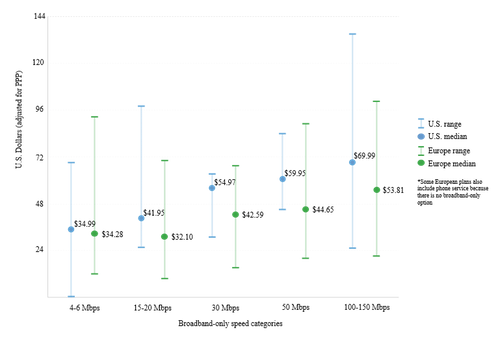
\includegraphics{comparison}
	\centering
\end{figure}

The plight of the American home Internet user is exposed even more when considering the highest available home Internet speeds for affordable Internet plans. While residents of Seoul and Hong Kong can choose among plans offering 300 Mbps connections in the price range of \$35-\$50, no American city has any plans offering > 50 Mbps speeds for the same price range. [cite connectivity] The much cheaper and faster connections available in Asia demonstrate that it is technologically feasible to provide fast home Internet connections for a low price. 

Not coincidentally, ISPs in Asia operate in a much more competitive landscape, forcing them to provide quality service at a lower price. In South Korea, for example, upstart ISPs can lease, and sell, unused bandwidth from a public utility that reaches the vast majority of the clustered, urban population. Further, the South Korean government forced Korea Telecom to open its network in the '90s, leading to increased competition and lower prices for users[cite wired]. 

Further, the population of the United States is large and spread out over a vast expanse of land. Reaching more homes in the United States requires laying lots of costly wire, which is often prohibitively expensive. Consider the efforts of Google Fiber. Google Fiber aims to offer connection speeds of 1000 Mbps at a comparable price to existing plans, reaching consumers in select neighborhoods of select American cities[cite google fiber]. According to Google, the process of bringing Fiber to a city involves initial exploration, network design, construction (laying fiber), and finally, customer sign up and installation. A Goldman Sachs report on Fiber, estimated that it would cost around \$140 billion for Google to cover the whole country[cite Goldman]. Further, the involved process required to dig and install fiber is extremely time consuming. The cost and time required to lay fiber across a wide geographic area makes it extremely difficult for even established companies like Google to enter the ISP realm, much less a host of smaller companies or startups. . In 2014, Tom Wheeler, Chairman of the FCC, acknowledged the lack of competition among ISPs and recognized a need for the FCC to do more to protect and create competition in the United States [cite Wheeler].

\subsection{A (Potential) Solution: Wireless Mesh Networks}
With the cost of establishing novel, last-mile wired networks being so high, there has been a lot of work on establishing wireless networks. One such notable project is Roofnet, a wireless mesh featuring over 40 nodes spread out over the urban area of Cambridge, Massachusetts. Roofnet nodes consist of a small PC, an 802.11b card, and an 8 dBi omni-directional antenna. These nodes are primarily installed on three to four story tall buildings, with packets hopping wireless nodes until they reach a wireless node which is also connected to a gateway to the rest of the wired Internet[cite roofnet]. Individual users install these nodes on their roofs or windows and join the network. 

Similar to Roofnet, another community powered mesh exists in Red Hook, Brooklyn[cite NYT Red Hook]. The goal of these networks is to provide a cheaper, more accessible form of Internet architecture in comparison to the extremely expensive deployment of fiber cables. However, these wireless networks face challenges operating in the urban environment.

\subsection{Challenges with Wireless: Propagation and Measurement}
The propagation of wireless signals in a noisy, obstacle-ridden urban environment often results in wireless networks operating below peak efficiency. Buildings and other environmental obstacles, such as trees, can greatly increase the path loss of a wireless link between two nodes. Then, establishing a line-of-sight (LOS) connection between two wireless links is important for low-loss links and robust wireless networks. However, the Fresnel Zone (an ellipsoid-shaped volume) around the LOS must also be clear of obstacles for optimally low path loss between a transmitter and receiver. 

Much work has been conducted on measurement campaigns of wireless signal propagation. Theodore S. Rapaport has conducted many such campaigns in a variety of settings in order to explore real-world propagation in different environments. For example, Rapaport, Durgin, and Xu's "Measurements and Models for Radio Path Loss and Penetration Loss In and Around Homes and Trees at 5.8GHz" conducted such a campaign in a suburban area. Signal strength measurement were taken by moving a receiver around a 1m square area and averaged to represent the path loss for a given room or outdoor location[cite Rappaport]. Such campaigns, while useful for sampling signal strength at key locations, don't give a complete understanding of signal strength over a space. 

Other campaigns have attempted to get a more complete measurement in an urban environment. A group of Brazilian researchers conducted a measurement campaign in Rio De Janeiro with a fixed transmitter on the window of an 8 story building. They built a receiver block with GPS and collected measurements by driving around streets surrounding the building housing the transmitter. GPS and signal strength measurements collected by the receiver block are joined to construct a map of measured signal strength at street level. While this may be useful for mobile Internet users at the street level, participants in a wireless mesh for home Internet may have receiver nodes at various heights, necessitating a more 3-D measurement of signal propagation in urban areas. Manual campaigns such as these use labor intensive techniques commonly referred to as "war walking" or "war driving"; these campaigns also have to be limited in scope due to the physical limitations of where measurements can be performed manually. 

Other measurement campaigns have attempted to measure 3-D signal propagations using drone technology. Drones offer several unique features that can make a measurement campaign more robust and complete than traditional static or manually measured campaigns. DroneSense was an automated 3-D wireless signal measurement campaign created by a team of researchers from Dartmouth. The DroneSense system autonomously traversed indoor spaces using visual reference markers which trace a path through a space. These reference markers are physically placed in a space and the drone uses its on-board camera and computer vision techniques to identify markers and use these markers to autonomously navigate through hallways and rooms. The drone's onboard wireless radio is used to measure signal strength.

\begin{figure}[h]
	\caption{Left: Continuous 2-D map of signal strength measurements in the streets of Rio de Janeiro (Authors). Right: DroneSense system navigating indoor space using reference points.}
	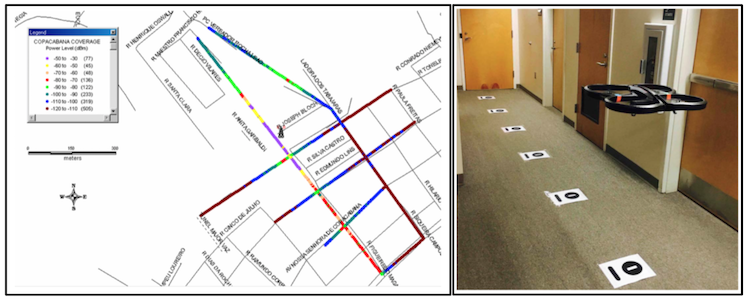
\includegraphics{related_work}
	\centering
\end{figure}

The DroneSense system can only measure signal strength in one frequency band because they rely on the drone's onboard wireless chipset; this doesn't allow the system to measure propagation under varying transmitter configurations. Regarding it's navigation module, DroneSense is limited in that it's navigation is reliant on physical reference points strategically arranged in 3-D space. This measurement technique is restricting in multiple ways. First, physical markers have to be created and laid out in 3-D space. While DroneSense is autonomous in terms of the drone's navigation, laying out the actual markers for the drone to navigate is still manual and limited by where markers can be placed. DroneSense also analyzes signal strength in terms of which reference point measurements were performed at. The reference points are points in 3-D space but do not have inherent spatial information encoded in them. Then, in addition to the manual placement of the reference points, DroneSense requires manual mapping of the reference points to 3-D space in order to create a continuous map of signal propagation. Lastly, DroneSense is limited to indoor measurement, where the measurement environment is much more contained and well behaved. 

\subsection{This Project: A More Robust Measurement Approach}
Common measurement techniques such as "war walking" and "war driving" don't provide robust, complete data that allow us to understand real-world signal propagation in complex urban environments. Newer approaches using drone technology, while promising due to spatially versatile, autonomous measurement, have also been limited in a variety of ways. Then, the question still remains: \textit{how can we gather more robust data to better inform the design of wireless mesh networks}?

Primarily, the data should help us form a complete picture of how a wireless signal from a transmitter propagates through a given environment. A crucial element of this is to perform measurements of signal strength in the complete 3-dimensional space. This is important because in a wireless mesh network, users may place transmitters and receivers in many different spatial configurations; for example, end users may live or work on different floors of apartment buildings and place antennas at varying heights. While DroneSense attempted to perform measurements in 3-D, their usage of reference points meant that their measurements were limited by the spatial arrangement of these points and the path the drone took to get to each of these points. Instead, a robust data set that would allow us to better understand real-world propagation would be a 3-D map of propagation through an environment.

Mesh networks can also be developed in many different environments. Dense urban environments with taller buildings may necessitate a propagation map with emphasis on the vertical space between buildings. More spread out suburban environments with shorter buildings may require require measurement over large swaths of land. A robust measurement technique should be easily configurable to perform measurements in a variety of different environmental configurations. This versatile method would  depart from the conventional methods of war walking and war driving; there are many environmental configurations where it would be extremely demanding or impossible for humans to be physically involved in the measurement process. For the measurement technique to operate without direct human input, it would likely have to navigate autonomously. Drones are growing increasingly technologically capable and accessible; this technology could be strategically used to perform truly 3-D measurements autonomously. 

A robust 3-D data set of signal strength measurements could help inform best practices for mesh network design. Experimental methodology is a  multi-faceted implementation choice that can greatly impact how insightful a signal propagation map can be towards real-world network configuration. Antennas in a mesh network can be placed in many different physical locations and operate with a variety of configurations. For example, transmitters can operate in different frequency bands depending on their circumstances. In urban environments, a signal in the 2.4GHz ISM band can provide better penetration through obstacles than a signal in the 5 GHz band; however, certain crowded channels in the 2.4 GHz may cause undesirable interference and require transmission in a less crowded channel. Experiments should account for these varying configurations and the measurement technique should also allow for measurement across commonly used ISM frequency bands. 

Lastly, there needs to be a digestible way to analyze the 3-D maps of signal strength across various experiments to determine which configurations worked better than others. This will require a combination of data visualization and data analysis. Visualizing the 3-D map can provide an intuitive understanding of how certain environmental features affect signal propagation in various configurations. Smoothing and aggregating the measured values over area or volume can provide metrics which help us digest the data and inform actual mesh network design.

\subsection{PROJECT ACRONYM: PROJECT TITLE}

Motivated by the desire to build more performant wireless mesh networks  in cities and suburbs, [PROJECT ACRONYM] aims to develop a robust measurement technique to measure signal propagation in urban environments. [PROJECT ACRONYM] will demonstrate the ability to create a 3-dimensional map of signal propagation in an urban environment; further, [PROJECT ACRONYM] will perform measurement experiments in different environments with various configurations to show how the versatility and extensibility of this measurement technique. Lastly, an analysis framework will be developed to show how the 3-dimensional maps of signal strength, in concert with various experimental setups, can actually guide real world mesh network design. 

To do this, we will build a signal measurement apparatus and fly it with a drone to conduct a measurement campaign in a handful of locations on the Princeton campus. A measurement apparatus collecting and storing signal strength measurements across the 2.4 GHz ISM band will be mounted on a drone. We will fly a drone on autonomous missions, where the drone will create accurate, high-resolution internal flight data logs; over the course of a flight, these flight logs will document the drone's latitude and longitude coordinates with 1 meter precision, along with the drone's height above ground. We will join the drone's flight log data with the measured signal strength data recorded on our measurement apparatus. This joined data set will let us create 3-dimensional point maps of signal strength at frequencies across the 2.4 GHz band. The collected data can then be aggregated to get a comprehensive, robust 3-dimensional map of signal strengths around a certain urban feature, such as a courtyard or a street with buildings on both sides.

There are two overarching research goals of this project. The first is to successfully generate a 3-D point cloud with associated signal strength measurements in an urban environment. This data set will serve as the foundation for the subsequent research goals of the project. Experiments will be ran with various transmitter locations and configurations, including varying center frequencies and channel widths; a separate 3-D point cloud generated for each experiment. These sets of experiments will be performed at a handful of locations across campus. Then, another important research goal of the project is to be able to spatially aggregate these point cloud data sets into "buckets", where each bucket is assigned a value equal to the average signal strength of point measurements in that bucket. This would serve multiple purposes, making the data more intuitively understood and easily visualized. Also, this would allow us to normalize the data per unit of volume; normalized values can help compare the effect of certain transmitter configurations and environmental features on propagation.

\begin{figure}[h]
	\caption{A mockup of the main research goals of [ACRONYM]. Left: A 3-D point cloud of signal strength measurements, given a fixed position transmitter. Right: After analysis and aggregation, spatial buckets of average signal strength values are formed; this normalized data can be compared across experiments with various configurations.}
	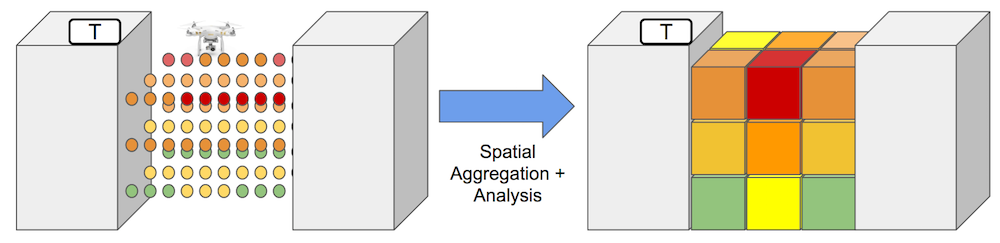
\includegraphics{measurement_goal}
	\centering
\end{figure}

This approach is novel because it would yield a robust, 3-dimensional map of signal propagation; existing measurement techniques are restricted to 2-dimensional maps or static point measurements. Additionally, using a drone to fly autonomous missions and collect measurements makes this approach viable in many different environments where war walking or war driving would be impossible. Since this project is motivated by wireless mesh networks,conducting measurements at various heights in challenging urban spaces is important as users can be situated at various floors. 
The analysis framework we propose allows us to normalize and compare these complete 3-D data sets across many configurations to determine how best to layout a mesh network in an environment with certain features.

The remainder of this work discusses how the technological stack required by this approach was designed and built, and then proceeds to detail the methods of data collection and experimentation. Finally, it attempts to show how the proposed spatial aggregation analysis can inform better mesh network design in the future.

\section{Implementation: Point Cloud of Signal Strength Measurements}
Several implementation challenges presented themselves as we began to work towards the primary research goal. The following sections describe how we built the various components required to construct a 3-D point cloud of signal strength measurements. Mainly, transmitter configuration and receiver apparatus design are  important design choices for any measurement campaign. The receiver apparatus had to measure and record signal strength over time and, importantly, be mountable on the drone. The drone then had to safely and autonomously fly with the measurement apparatus attached. The spatial data recorded by the drone had to be joined with the data collected by the receiver apparatus to generate the 3-D point cloud.

\subsection{Part 1: Transmitting a Wireless Signal}

\subsubsection{Transmitter Selection}
Since this project was focused on measuring the performance of wireless networks in urban environments, it was imperative to choose a transmitter which would be typically used in an urban setting. Consider a mesh network configuration in a town such as Princeton. This mesh network would need to meet several key criteria. First, it would need to have a way to connect to the wired Internet at some wired gateway, which could be many miles away or even in another town altogether. One reasonable way to establish this connection would be with the use of high-throughput, carrier-grade, long-range backhaul links which can establish wireless connections at ranges upwards of 100 km [Ubiquiti cite].

End users of the mesh network living in Princeton would not be connecting directly to these backhaul links, however. Backhaul links would need to be placed at high elevations and meticulously aligned with one another to establish a LOS connection. It may be impossible for users to establish LOS connections with backhaul links because users will often have windows or roofs with obstructed views; further, they will also have pyhsically smaller, lower power antennas where they may not be able to transmit to a distant backhaul link.

Instead, a third kind of antenna is required to fill in the gaps between user bridge antennas and powerful backhaul links. A Point-to-Multi-Point (PtMP) link, which transmits to several receiving antennas, is required to complete the mesh network configuration. These PtMP links are more cost effective and smaller than backhaul links; they can be placed around the town of Princeton and serve as connection points for the end users who live on the same street, housing development, or intersection as one of these links.

For this project, the Ubiquiti NanoStation M2 will be used; the NSM2 is a PtMP link which operates in the 2.4GHz spectrum. The NSM2 is appropriate for an urban mesh network because it has good 180-degree coverage in the azimuth and elevation planes. Then, if it is placed on top of a building facing the street, it can ideally provide a strong signal to a number of other buildings on the same street at a variety of elevations (floors); a large number of users would be able to connect to the locoM2 from their windows and join the wireless mesh.

\begin{figure}[h]
	\caption{Radiation patterns of the Ubiquiti NanoStation M2}
	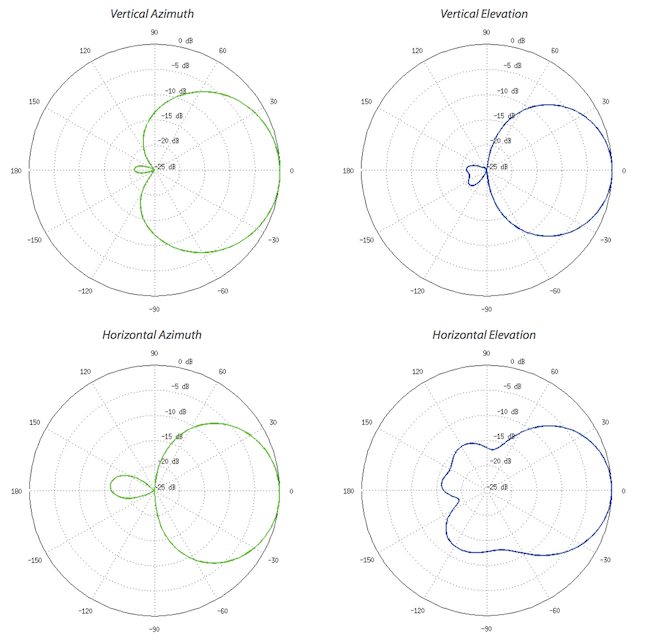
\includegraphics{nsm2_radiation}
	\centering
\end{figure}

\subsubsection{Transmitter Selection}

Ubiquiti transmitters also allow for fast and easy configuration through the built-in airOS operating system. The airOS interface is accessed through a web browser and allows the user to change the operating mode of the device, the channel width, and the center frequency of the device; these parameters will be varied during the experimentation phase. For this implementation the Ubiquiti transmitter will receive power-over-ethernet (PoE) from a portable power supply and PoE adapter. The transmitter will also be mounted on a telescoping tripod, which will allow us to experiment with the transmitter at various heights if it's not possible to move between floors.

\subsection{Part 2: Measuring Wireless Signals in 3-D}
In order to create a 3-D point cloud of signal strength measurements, measured values need to be combined with 3-D spatial data. Two major implementation components are needed to achieve this goal. First, a drone is required to collect spatial data across various planes at many different heights. A signal measurement apparatus which can detect signals  across the 2.4GHz spectrum and then record these measurements is also needed. If this apparatus can somehow be mounted on the drone, we could feasibly gather wireless signal data throughout a 3-D space. The data collected on these separate devices  can then be joined into a single data set representing the 3-D point cloud of signal strength measurements. 

\subsubsection{3-Dimensional Data: Collected via Drone}
Collecting precise and accurate spatial data would only be possible if a reliable  drone with state-of-the-art battery life could both log flight data and be autonomously controlled. Autonomous control is imperative to fly the drone in specific flight patterns, which can be overlayed on each other to produce the robust, complete dataset required for the 3-D point cloud. The DJI Phantom 3 Advanced is a "pro-sumer" drone which produces incredibly precise spatial data using multiple built-in stability and guidance systems. DJI is a world-leader in producing drones for hobbyists as well as professionals. While other companies such as Parrot Drones sell devices with open-source hardware and software for increased customizability, this project used a DJI drone which was less customizable but more reliable. Reliability and fault-tolerance was a key consideration because drone flights would be conducted in urban settings more prone to signal interference where drone failure could cause harm to property or people. Further, because of DJI's large market share, many third party apps leverage the extra features of the Phantom 3 Advanced that would potentially have to be created separately if another brand was used. 

Battery life was an important consideration because many autonomous flights would have to be conducted in a given space, each lasting several minutes. With an approximate 23 minutes of flight time out of the box, the P3A offers one of the longest flight times available in the consumer drone space. The P3A was used instead of the Phantom 4, a more recent model, because it has has a removable camera gimbal which was leveraged to build a mounting bracket housing the measurement apparatus (see Measurement Apparatus section, Mounting section). 

\subsubsection{Spatial Data Collection}
The P3A features an optical stabilization system for micro-level positional adjustments and a robust satellite positioning system for macro-level navigation purposes. DJI's "Vision Positioning System" (VPS) features two ultrasonic sensors and a monocular camera on the bottom-side of the drone.These sensors are always-on and the P3A uses the ultrasonic devices to measure distance from the ground and the camera to identify patterns under the drone; this input can be used to stabilize the drone such that it can hover in place or closely follow a pre-defined path. On the other hand, the P3A's satellite positioning system uses both GPS and GLONASS (the Russian satellite network) to provide geographic location services. The inclusion of GLONASS effectively doubles the number of satellites the P3A can fix onto; throughout testing and experimentation, the P3A was regularly fixed with 14+ satellites, providing robust, 1 meter accuracy. The geographic coordinates and the height measurements gathered by the satellite position system and VPS, respectively, are logged on automatically created flight logs and also transmitted to the drone's controller in real-time.

\subsubsection{Precision and Automation: Litchi iOS app}
Many third-party apps take advantage of these systems to provide autonomous navigation on the P3A. Litchi is an app which features a "Waypoint" mode where users can construct a path out of waypoints for the drone to follow. Custom heights and speeds can also be set for the waypoints; the drone's heading can also be manually controlled along the route. Specifically, Litchi allows the user to control the drone's heading using "points of interest"; for this project, the location of the transmitter will be a POI the drone will orient towards. At the start of a waypoint mission, the entire path is wirelessly uploaded to the drone which performs an auto-takeoff maneuver to begin the autonomous mission. The drone travels from it's starting location to the first waypoint and continues to follow the path until it reaches the last waypoint. 

\begin{figure}[h]
	\caption{Left: Waypoint mode in the Litchi app, viewing a mission. Purple markers denote the waypoints, which the drone will traverse in numbered order. The clouds above each marker indicate the height the drone should assume at a given waypoint. The opaque blue paper airplanes under the waypoints indicate the drone's heading. The blue marker is a point of interest. Right: Path followed by the drone during a test of this waypoint mission; the drone took from the H (home) marker. Note that waypoints are separated by < 16 ft, demonstrating the granular position control of Waypoint mode.}
	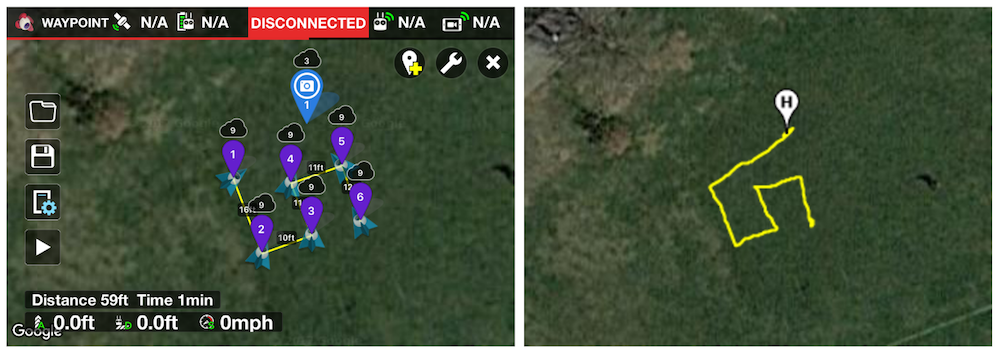
\includegraphics{waypoint}
	\centering
\end{figure}



\subsection{Receiver Apparatus Overview}
The design of the receiver apparatus was heavily constrained by weight. In total, the receiver apparatus weighted (TODO: X). If we were to mount the apparatus on a drone, it would certainly need to be light enough for the drone to fly and be controlled reliably. Another important constraint was the ability to interface with the equipment, since the various dimensions of the collected data needed to be logged for later analysis.

The receiver apparatus had to accomplish several key functions in order to gather the 3-D data required to meet the primary research goal. At a high level, the receiver apparatus would need to simultaneously log signal strength and GPS measurements, joining these measurements together as single rows of data. Then, height data could be joined to provide the basis for constructing a 3-D map of wireless signal propagation in a given area; analyzing the data from this map could inform best practices for transmitter and/or receiver placement in various urban settings.

The receiver apparatus was built on cardboard and contained a Raspberry Pi, spectrum analyzer, GPS module, GPS external antenna, and a portable battery pack; a measurement and logging script ran on the Raspberry Pi. The following sections describe each of these design elements in more detail.

\begin{figure}[h]
	\caption{Layout of the receiver apparatus, which is to be mounted on a DJI Phantom 3 drone.}
	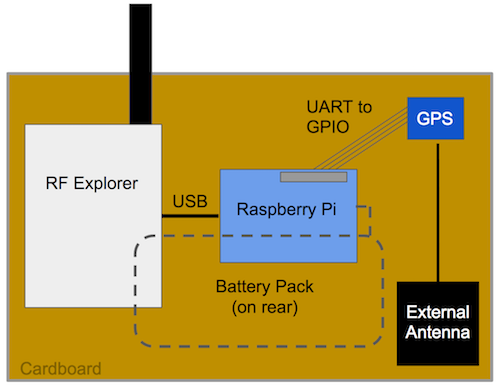
\includegraphics{apparatus}
	\centering
\end{figure}

\subsection{On-board Computing and Logging}
A Raspberry Pi 2 Model B served as the on-board computer of the receiver apparatus. The Raspberry Pi was selected for it's versatile interfacing options and expandable flash storage, as well as it's very light weight (TODO: weight), power efficient design (200mA operating current). Specifically, the Model B has 4 built-in USB ports as well as 40 General Purpose Input/Output (GPIO) pins. This meant that we could connect multiple pieces of equipment to the apparatus and also maintain the ability to finely configure equipment by connecting via GPIO. The Pi ran a Raspbian Jessie operating system mounted on a 64 GB SD card, which stored the collected data. To power the Raspberry Pi, a lightweight (254 g) battery with a max output of 5V, 3.4 Amps was used. 

\subsection{Spectrum Analyzer}
The receiver apparatus needed to have an actual receiver to measure the strength of wireless signals in the 2.4GHz. This project used the RF Explorer handheld spectrum analyzer, a lightweight spectrum analyzer (185g) that can run off it's own internal battery [cite Seeedstudio].\\
To collect data from the RF Explorer, the RF Explorer was connected to a Raspberry Pi(see "Logging and Compute") with a serial connection over USB. The RF explorer sends bits over the serial connection; these bits are structured as "sweeps" of signal measurement data. On each sweep, RF Explorer sends the measured signal strength for frequencies from 2412 MHz to 2472 MHz[EDIT], which correspond to the center frequencies of channel 1 and channel 13 under the 2.4 GHz Wi-Fi protocols.

RF-Explorer-For-Python (RFEP) is a Python library with an API for detecting, connecting to, and reading from an RF Explorer device. Upon instantiating a RFECommunicator object provided by RFEP, the user can connect to the RF Explorer by configuring the RFECommunicator connection as a serial connection with the appropriate USB device port. The RFECommunicator then provides utility functions to read sweeps of data, returned as arrays of length [TODO: X] with frequency steps of [TODO: Y] MHz. This functionality will allow us to simultaneously gather and log signal strength data across the transmitting frequencies of our PtMP link, as determined by the transmitter's configured center frequency and channel width.

[TODO: Stripping Weight off RFE]

\subsection{GPS Module}
GPS positional measurement would be required to construct the 3-Dimensional map of signal propagation. While the drone being used to perform the data, the DJI Phantom 4, logs its own on-board GPS data, the receiver apparatus needed its own dedicated GPS logging to coordinate the simultaneous logging of both signal strength measurements and GPS coordinates; using dedicated modules connected to the same Raspberry Pi would be the most straightforward implementation choice to accomplish this. Additionally, the GPS module would have to be very sensitive as the 3-Dimensional signal propagation maps would be constructed around urban features; in order for the maps to be insightful, positional data would need to be sensitive to a few feet.

The Adafruit Ultimate GPS Breakout board was used, which featured 10 Hz updates and weighed only 3.5g. It also operated with a very low current draw of 25mA. The Breakout could only be interfaced through a universal asynchronous receiver/transmitter (UART) device; the Raspberry Pi was connected to the GPS UART using the Pi's GPIO pins, establishing a serial connection. With weight and connectivity accounted for, the GPS module still needed to be accurate at high resolution. Through initial testing runs, the GPS Breakout board on it's own proved to be inaccurate. To provide additional signal gain and increase the reliability of positional data, the Adafruit external GPS antenna was added to the receiver apparatus.  

\subsection{Measurement and Logging Script}
[TODO: Rework]

In order to construct the 3-Dimensional map of signal propagation, the receiver apparatus would need to simultaneously gather data from the spectrum analyzer and the GPS module and log this data in the Raspberry Pi's onboard filesystem. As mentioned earlier, both the spectrum analyzer and GPS module communicate with the Pi over serial connections; this posed a challenge because of two separate methods used to read serial data that was being transmitted at different baud rates.

First, data from the RF Explorer was collected at 50000 baud via the USB serial connection using the RFECommunicator object from the RFEP library. The RFECommunicator object featured several convenient utility methods to get parsed signal strength data in an array. The GPS module, however, was connected to the Raspberry via the GPIO pins; data from the Adafruit GPS Breakout module was collected at 9600 baud using the pySerial library. These approaches worked in isolation but resulted in an infinitely hanging process when combined

Based on specifics of the libraries being used, it was cumbersome to read from both serial connections in the same process. Specifically, the methods used were blocking on their respective serial ports. This was an issue because the two devices were sending data at different baud rates; accommodating a blocking read from either device, would result in not reading some amount of serial bits from the other device. To avoid this issue, the measurement script read from the RFExplorer's serial port and spawned a child thread to read from the GPS via Python's Threading library. Then, global variables for relevant GPS data were initialized in the parent thread and the spawned GPS thread would simply populate these global variables as data was available on the serial connection.

Data was logged in the parent process after every new sweep of data is received from the RF Explorer. Because of the multi-threading approach, the process logs the most recently collected GPS data. Data is logged as rows in a CSV file in the following format: \texttt{time, frequency, dBm, latitude, longitude}. Time corresponds to how long the script has been running, while latitude and longitude are positional coordinates in degrees and minutes format. The script takes arguments to determine for which frequencies to record measured signal strength values (in dBm); the script takes the transmitters center frequency and channel width as arguments. For each signal strength measurement that falls within this band of frequencies, the script logs a row of data.  


\end{document}

